\documentclass[11pt,reqno]{amsart}
\usepackage[T1]{fontenc}
\usepackage{lmodern,amsmath,amssymb,amsthm,mathtools,microtype}
\usepackage[a4paper,margin=28mm]{geometry}
\usepackage{xcolor,tikz,booktabs,enumitem,needspace}
\usetikzlibrary{arrows.meta,positioning,calc}
\definecolor{deepteal}{RGB}{15,81,85}
\usepackage[colorlinks=true,linkcolor=deepteal,citecolor=deepteal,urlcolor=deepteal]{hyperref}
\usepackage[nameinlink,noabbrev]{cleveref}
\numberwithin{equation}{section}
\newtheorem{theorem}{Theorem}[section]
\newtheorem{proposition}[theorem]{Proposition}
\newtheorem{lemma}[theorem]{Lemma}
\newtheorem{corollary}[theorem]{Corollary}
\theoremstyle{definition}
\newtheorem{definition}[theorem]{Definition}
\newtheorem{hypothesis}[theorem]{Hypothesis}
\newtheorem{example}[theorem]{Example}
\theoremstyle{remark}
\newtheorem{remark}[theorem]{Remark}
\newcommand{\E}{\mathbb E}
\newcommand{\Pp}{\mathbb P}
\newcommand{\one}{\mathbf1}
\newcommand{\eps}{\varepsilon}
\newcommand{\co}{\mathrm{co}}
\newcommand{\tr}{\tau}
\newcommand{\TV}{d_{\mathrm{TV}}}
\newcommand{\supp}{\operatorname{supp}}
\newcommand{\rank}{\operatorname{rank}}
\newcommand{\PhiK}{\Phi_K}
\newcommand{\norm}[1]{\lVert#1\rVert}
\newcommand{\abs}[1]{\lvert#1\rvert}
\newcommand{\FR}{\mathsf{FR}}
\DeclareMathOperator{\Ent}{H}
\setlist[enumerate]{label=\textup{(\roman*)},leftmargin=*,itemsep=3pt}
\setlist[itemize]{leftmargin=*,itemsep=3pt}
\hypersetup{pdftitle={Entropy Budgets and Weighted Concentration in Parallel Games},pdfauthor={Harjas Sandhu}}
\title[Entropy budgets in parallel games]{Entropy Budgets and Weighted Concentration\\in Parallel Games}
\author{Harjas Sandhu}
\address{The University of Queensland}
\email{harjas.sandhu@student.uq.edu.au}
\date{6 November 2026}
\subjclass[2020]{Primary 60E15, 68Q17; Secondary 46L53, 81P45, 94A17}
\keywords{parallel repetition, weighted concentration, conditional entropy, commuting strategies, positive factorization, common information}
\begin{document}
\raggedbottom
\begin{abstract}
We prove a concentration principle for arbitrarily correlated binary success indicators satisfying an explicit conditional entropy budget, with parameters \(K\ge1\) and \(C_0\ge0\). If the benchmark losses are \(\eps_i\), the natural scale is \(S=\sum_i\eps_i^2\), and the probability that the weighted loss \(\sum_i\eps_i(1-W_i)\) is at most \((1-r)S\) is bounded by \(\exp[-r^5S/(2^{21}K^4(1+C_0))]\). The proof uses independent sparse success tests, an exact posterior entropy identity and a differential bound, and applies at every finite length. Under a separately stated finite-tracial reconstruction hypothesis, the principle gives heterogeneous commuting-game bounds for disjoint-block predicates, including projection predicates, and a charged extension. We also identify the exact limitation of positive-factor mass bounds: outside the disjoint-block class, global tensor factorizations can require exponential mass even at success probability one. A robust common-information argument rules out uniformly low-mass accurate filters on all near-perfect tested instances. Nevertheless independent question-free nuisance registers cancel exactly from entropy increments. This separates an obstruction to positive-mass reconstruction from the unresolved problem of controlling entropy directly for general correlated strategies.
\end{abstract}
\maketitle

% Begin introduction.tex
\section{Introduction}
Parallel repetition asks whether joint strategies can defeat repeated tests more effectively than independent play. The questions in different coordinates may be independent while the answers, and hence the successes, are highly correlated. A proof of exponential decay must control those correlations rather than assume them away.

This paper isolates a conditional information principle behind such arguments. Testing a set of coordinates and learning that they all succeeded changes the distribution of the untested coordinates. Suppose that the total reconstruction deficit of the remaining coordinates is bounded by the logarithmic cost of that conditioning, together with a charge for the tested predicates. We show that this information budget forces concentration of a weighted loss. The tests may differ in every coordinate, and their individual squared gaps accumulate.

There are two distinct mathematical statements. The main theorem is a finite-probability implication from a precisely defined budget to concentration. Its proof is self-contained and makes no operator-algebra assumption. The commuting-game application assumes a finite-tracial coordinate reconstruction property, stated explicitly in \cref{hyp:FR}. We prove that this property supplies the scalar budget and explain the passage to arbitrary commuting tables using Lin's density theorem. We do not assert the reconstruction property as an unconditional theorem of this paper.

\subsection{The concentration statement}
Let \(W_1,\ldots,W_N\) be binary success indicators on one probability space, with an arbitrary joint law. Fix benchmark losses \(\eps_i\in[0,1]\), nonnegative charges \(\kappa_i\), and \(K\ge1\). For \(D\subseteq[N]\), write
\[
 E_D=\{W_j=1\text{ for every }j\in D\},\qquad p_D=\Pp(E_D).
\]
When \(p_D>0\), define the conditional losses
\[
 \alpha_i(D)=\Pp(W_i=0\mid E_D),\qquad i\notin D.
\]
The continuous deficit function is
\begin{equation}\label{eq:phi}
 \PhiK(e,a)=
 \left[\frac{\sqrt{a+4(e-a)_+/K}-\sqrt a}{2}\right]^4,
 \qquad x_+=\max\{x,0\}.
\end{equation}
It is the exact inverse of the fourth-root error relation used below. In particular it vanishes when the conditional loss is already at least its benchmark.

We use \(\Ent\) and \(I\) for Shannon entropy and mutual information in natural units, \(D(P\Vert Q)=\sum_xP(x)\log(P(x)/Q(x))\) for relative entropy, and \(\TV(P,Q)=\frac12\sum_x|P(x)-Q(x)|\) for total variation. The value \(D(P\Vert Q)\) is infinite when \(P\) is not supported on the support of \(Q\).

\begin{definition}[Conditional entropy budget]\label{def:budget}
The law of \(W=(W_i)_{i=1}^N\) satisfies the budget with parameters \((\eps_i,\kappa_i,K)\) if every proper \(D\subsetneq[N]\) with \(p_D>0\) obeys
\begin{equation}\label{eq:budget}
 \sum_{i\notin D}\PhiK(\eps_i,\alpha_i(D))
 \le 3\log(1/p_D)+2\sum_{j\in D}\kappa_j.
\end{equation}
All logarithms are natural. No conditional probability is assigned to an event of probability zero.
\end{definition}

\begin{theorem}[Weighted concentration]\label{thm:main}
Assume \cref{def:budget}, and suppose that
\(\kappa_i\le C_0\eps_i\) for some \(C_0\ge0\). Set
\[
 S=\sum_{i=1}^N\eps_i^2,\qquad
 Z=\sum_{i=1}^N\eps_i(1-W_i).
\]
If \(S>0\), then, for every \(0<r\le1\),
\begin{equation}\label{eq:main}
 \Pp\{Z\le(1-r)S\}
 \le \exp\left[-\frac{r^5S}{2^{21}K^4(1+C_0)}\right].
\end{equation}
For \(S=0\), the corresponding bound is one. The result holds for every finite \(N\ge1\).
\end{theorem}

The benchmarks need not be the actual marginal losses. The budget itself implies \(\Pp(W_i=0)\ge\eps_i\): take \(D=\varnothing\) in \eqref{eq:budget}. Thus \(S\) is a lower bound on the mean of \(Z\). The conclusion concerns a lower tail below that reference level.

\begin{example}[Which failures does the weighted event permit?]\label{ex:weights}
Take \(\eps=(1/2,1/4,1/8,0)\). Then
\[
 S=\frac{21}{64},\qquad
 Z=\frac12(1-W_1)+\frac14(1-W_2)+\frac18(1-W_3).
\]
At \(r=1/2\), the event \(Z\le21/128\) is exactly
\(\{W_1=W_2=1\}\). The third coordinate may fail; the fourth has zero weight. For independent losses with means \(\eps_i\), every conditional deficit is zero, so the budget holds with all charges zero. In that example the event has probability \(3/8\). The universal constant in \eqref{eq:main} is deliberately conservative and is not intended as a sharp estimate for a four-coordinate experiment.
\end{example}

The budget is substantially stronger than a condition on the means. For \(0<\eps<1\), if all \(W_i\) equal the same Bernoulli variable with success probability \(1-\eps\), their marginal losses are \(\eps\), but their all-wins probability remains \(1-\eps\). After conditioning on one win, every remaining loss is zero. Since \(\PhiK(\eps,0)=\eps^2/K^2\), zero-charge budget \eqref{eq:budget} fails for large \(N\). This simple example explains why a genuine conditional hypothesis is necessary.

A second, shorter argument gives a better constant at the all-wins endpoint.
\begin{theorem}[All wins]\label{thm:allwins}
Under the hypotheses of \cref{thm:main}, put \(t_0=1/(256K^4)\). Then
\begin{equation}\label{eq:allwins}
 \Pp(E_{[N]})\le
 \exp\left[-\frac{t_0}{3+4C_0+2t_0}\sum_i\eps_i^2\right].
\end{equation}
\end{theorem}
The proof is given in \cref{sec:allwins}. Neither theorem assumes independence of the \(W_i\), an attained optimization problem, or an asymptotically large product length.

\subsection{Reconstruction, obstruction and cancellation}
In a nonlocal game, \(\eps_i\) can be the gap \(1-\omega_{\co}(G_i)\). The additional task is to prove \eqref{eq:budget} for every joint strategy. We state the exact reconstruction hypothesis needed for this task in \cref{sec:games}. It includes local legality on every input pair and does not assert finite-matrix density. Disjoint-block winning relations have zero presentation charge; ordinary projection predicates belong to this class.

The rest of the paper studies the limits of obtaining such a budget from positive factorizations of an accepting predicate. We prove three complementary facts. First, disjoint-block masks are the maximal class with a uniform subexponential positive-mass guarantee. Second, even approximate filters cannot satisfy a universal low-mass requirement on all near-perfect tested instances. Third, independent nuisance registers nevertheless cancel exactly from exposure entropy increments. The third fact repairs the padding examples used in the first two: a large endpoint normalization need not create a large entropy change.

\subsection{Relation to earlier methods}
Classical parallel repetition begins with Raz and Holenstein \cite{Raz,Holenstein}; Rao obtained projection repetition and concentration estimates \cite{Rao}. Weighted concentration for correlated variables and random-subset conversions from direct products to thresholds have earlier forms in Unger and Impagliazzo--Kabanets \cite{Unger,IK}. Our scalar contribution is the implication from \eqref{eq:budget}, including its logarithmic successful-test cost, to a heterogeneous weighted tail. It is not a claim that weighted concentration or random subset testing was previously unknown.

For unique games, the semidefinite programming method of Kempe--Regev--Toner already supplies quadratic-gap products \cite{KRT}. Classical and entangled projection products have powerful analytic treatments \cite{DS,DSV}. General tensor-game cubic bounds and conditional-relative-entropy methods provide further comparisons \cite{Song,Jain}; they do not by themselves supply the finite-tracial reconstruction hypothesis used here. Lin proves an anchored commuting repetition theorem and the classification \(\mathsf{MIP}^{\co}=\mathsf{coRE}\) \cite{LinMIP}. Neither a new complexity classification nor an unqualified general quadratic commuting repetition theorem is claimed here.

Positive predicate decompositions and their Markov separators also have explicit predecessors in Holenstein's Section~8 \cite{Holenstein}. The scatter common-information formula used in our obstruction is established work of Cuff--Permuter--Cover and Cuff \cite{CPC,Cuff}. We give the relevant finite proofs and separate these ingredients from the budget implication and the reconstruction obstruction developed below.

% End introduction.tex

\clearpage

% Begin overview.tex
\section{The mechanism in one page}\label{sec:overview}
The probability argument can be understood without first entering the commuting model. Its starting point is the scalar budget \eqref{eq:budget}. In the game application, local reconstruction is the additional operation that must supply this budget.

\begin{center}
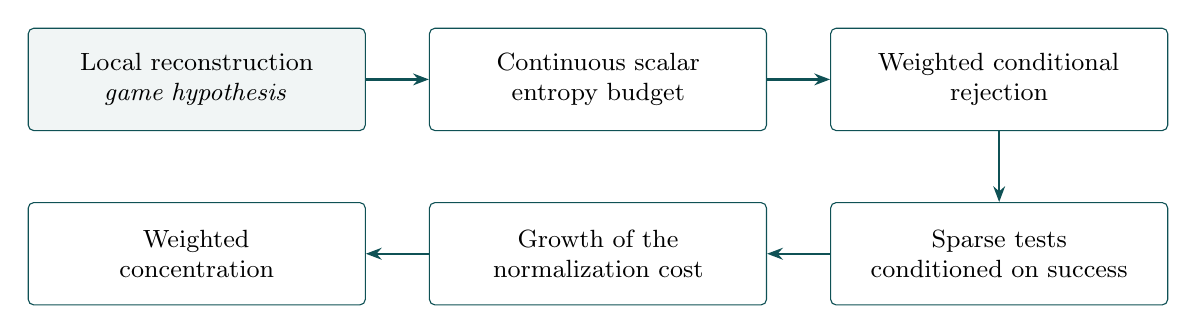
\begin{tikzpicture}[
 box/.style={draw=deepteal,rounded corners=2pt,align=center,
 text width=40mm,minimum height=13mm,font=\small,inner sep=4pt},
 arr/.style={-{Stealth[length=2mm]},thick,deepteal},
 node distance=9mm and 8mm]
 \node[box,fill=deepteal!6] (rec) {Local reconstruction\\\emph{game hypothesis}};
 \node[box,right=of rec] (bud) {Continuous scalar\\entropy budget};
 \node[box,right=of bud] (loss) {Weighted conditional\\rejection};
 \node[box,below=of loss] (tilt) {Sparse tests\\conditioned on success};
 \node[box,left=of tilt] (bar) {Growth of the\\normalization cost};
 \node[box,left=of bar] (tail) {Weighted\\concentration};
 \draw[arr] (rec)--(bud);
 \draw[arr] (bud)--(loss);
 \draw[arr] (loss)--(tilt);
 \draw[arr] (tilt)--(bar);
 \draw[arr] (bar)--(tail);
\end{tikzpicture}
\end{center}

\paragraph{A conditional budget.}
After a tested set succeeds, some untested coordinates might become much easier. The left side of \eqref{eq:budget} measures that total deficit. Its right side charges the rarity of the tested success, through \(\log(1/p_D)\), and the structure of the tested predicates, through \(\sum_D\kappa_j\).

\paragraph{Why squared gaps appear.}
Multiply the one-coordinate reconstruction inequality by \(\eps_i\). Hölder's inequality combines the resulting errors through \(\sum_i\eps_i^2=S\). The natural statistic is therefore the weighted loss \(Z\), not an unweighted count of failures. This retains the contribution of each difficult coordinate even when many other tests have small gaps.

\paragraph{A soft way to favor successful outcomes.}
Choose a coordinate for testing with odds \(u\eps_i\), independently of the original experiment. Keep only runs in which every chosen coordinate wins. For a fixed loss pattern, the chance of surviving this auxiliary test is
\[
 f_u(W)=\prod_i(1+u\eps_i)^{-(1-W_i)}.
\]
Patterns with fewer weighted losses survive more often. The normalizer \(F(u)=\E f_u(W)\) is a soft lower-tail transform. Independence belongs to the auxiliary test choices; the original successes remain arbitrarily correlated.

\paragraph{The differential step.}
Let \(\ell(u)=-\log F(u)\). Its derivative is an expectation of weighted rejection under the tilted law. If \(\ell\) stayed small, the budget would force that tilted law to retain nearly the reference rejection \(S\). Its derivative would then remain large. Integrating over a short interval proves that \(\ell\) cannot be too small, and the lower-tail estimate follows.

\paragraph{Why factorization obstructions do not end the argument.}
A positive decomposition can carry a large shared label even when the accepting event is almost certain. That obstructs a low endpoint-mass estimate. However, a label independent of everything being exposed contributes the same entropy at every stage. Its contribution disappears on taking differences. The exact cancellation in \cref{sec:cancellation} makes this distinction explicit.

% End overview.tex

\clearpage

% Begin concentration.tex
\section{Sparse success tests and weighted concentration}\label{sec:proof}
We now prove \cref{thm:main}. All variables in this section are classical and finite. The success law is arbitrary apart from \eqref{eq:budget}.

\subsection{From individual deficits to weighted rejection}
\begin{lemma}[Exact inversion]\label{lem:inverse}
For \(e,a\in[0,1]\) and \(t\ge0\),
\[
 e\le a+K(\sqrt a\,t^{1/4}+\sqrt t)
 \quad\Longrightarrow\quad \PhiK(e,a)\le t.
 \]
If \(t=\PhiK(e,a)\) and \(a'=\min(a,e)\), then
\[
 e=a'+K(\sqrt{a'}\,t^{1/4}+\sqrt t).
\]
\end{lemma}
\begin{proof}
For \(a<e\), solve \(z^2+\sqrt a\,z=(e-a)/K\) for its nonnegative root and set \(t=z^4\). The polynomial is increasing for \(z\ge0\). For \(a\ge e\), \(\PhiK(e,a)=0\) and \(a'=e\). These two cases give both assertions.
\end{proof}

For any tested set \(D\) with \(p_D>0\), abbreviate
\[
 S_D=\sum_{i\notin D}\eps_i^2,\quad
 A_D=\sum_{i\notin D}\eps_i\alpha_i(D),\quad
 M_D=3\log(1/p_D)+2\sum_{j\in D}\kappa_j.
\]
For \(D=[N]\) define \(S_D=A_D=0\). The budget then extends automatically to this set by an empty sum; no reconstruction or conditional loss on a live coordinate is needed.

\begin{lemma}[Conditional weighted rejection]\label{lem:weighted}
For every \(D\) with \(p_D>0\),
\begin{equation}\label{eq:weighted}
 A_D\ge S_D-K\bigl(S_D^{3/4}M_D^{1/4}+\sqrt{S_DM_D}\bigr).
\end{equation}
\end{lemma}
\begin{proof}
For a proper set, put \(t_i=\PhiK(\eps_i,\alpha_i(D))\) and
\(\alpha'_i=\min(\alpha_i(D),\eps_i)\). By \cref{lem:inverse},
\[
 \eps_i=\alpha'_i+
 K(\sqrt{\alpha'_i}\,t_i^{1/4}+\sqrt{t_i}).
\]
After multiplication by \(\eps_i\), the uncapped sum \(A_D\) dominates the capped loss term. Since \(\alpha'_i\le\eps_i\), Hölder and Cauchy--Schwarz give
\begin{align*}
 \sum_{i\notin D}\eps_i\sqrt{\alpha'_i}\,t_i^{1/4}
 &\le \sum_{i\notin D}\eps_i^{3/2}t_i^{1/4}
 \le S_D^{3/4}\left(\sum_{i\notin D}t_i\right)^{1/4},\\
 \sum_{i\notin D}\eps_i\sqrt{t_i}
 &\le\sqrt{S_D\sum_{i\notin D}t_i}.
\end{align*}
Use the budget to bound the sum of \(t_i\). For the full set the assertion is \(0\ge0\).
\end{proof}
The cap in this proof is not a cosmetic simplification. Conditional losses can exceed their benchmarks; replacing \(\sqrt{\alpha_i}\) by \(\sqrt{\eps_i}\) without the exact inversion would be invalid.

\subsection{An auxiliary subset and its posterior}
For \(u>0\), include \(i\) in an auxiliary subset \(D\) independently with probability
\begin{equation}\label{eq:testodds}
 q_i(u)=\frac{u\eps_i}{1+u\eps_i}.
\end{equation}
The odds \(q_i/(1-q_i)=u\eps_i\) explain this particular choice: a failure is penalized by the simple factor \((1+u\eps_i)^{-1}\). Denote the product subset law by \(\nu_u\).

\Needspace{11\baselineskip}
\begin{lemma}[Successful-subset tilt]\label{lem:tilt}
Define
\[
 F(u)=\sum_D\nu_u(D)p_D,\qquad \ell(u)=-\log F(u).
\]
Then
\begin{equation}\label{eq:transform}
 F(u)=\E\prod_i(1+u\eps_i)^{-(1-W_i)}>0.
\end{equation}
Conditioning the joint subset/outcome experiment on \(E_D\) gives subset law
\[
 w_u(D)=\frac{\nu_u(D)p_D}{F(u)}
\]
and outcome law \(T_u\), the original law tilted by the product in \eqref{eq:transform}. Under this joint posterior, given the outcome, a losing coordinate is never selected and a winning coordinate is selected independently with probability \(q_i(u)\).
\end{lemma}
\begin{proof}
For a fixed outcome, every chosen coordinate wins precisely when no losing coordinate is chosen. Its probability is
\(\prod_{i:W_i=0}(1-q_i)=\prod_i(1+u\eps_i)^{-(1-W_i)}\).
Averaging proves \eqref{eq:transform}; its integrand is strictly positive. Bayes' formula gives the posterior subset law and the tilted outcome law. Success conditioning fixes each losing selection to zero and puts no additional restriction on a winning selection, proving the last assertion.
\end{proof}

\begin{example}[A correlated law, with all normalizations visible]\label{ex:tilt}
Let \(\eps=(1/2,1/4)\), and give outcomes \((1,1),(1,0),(0,1)\) probabilities \(1/4,1/4,1/2\). Every conditional loss is at least its benchmark, so \eqref{eq:budget} holds with zero charges. At \(u=1\), \(q_1=1/3,q_2=1/5\), and
\begin{center}
\begin{tabular}{lrrrr}
\toprule
\(D\)&\(\varnothing\)&\(\{1\}\)&\(\{2\}\)&\(\{1,2\}\)\\
\midrule
\(\nu_1(D)\)&\(8/15\)&\(4/15\)&\(2/15\)&\(1/15\)\\
\(p_D\)&\(1\)&\(1/2\)&\(3/4\)&\(1/4\)\\
\(w_1(D)\)&\(32/47\)&\(8/47\)&\(6/47\)&\(1/47\)\\
\bottomrule
\end{tabular}
\end{center}
Here \(F(1)=47/60\). The tilted outcome probabilities are
\((15,12,20)/47\), and
\[
 \E_{T_1}Z=\frac{13}{47}=\E_{w_1}A_D.
\]
Thus the subset posterior and the outcome tilt describe the same conditioning experiment. The proof will use much smaller \(u\); \(u=1\) makes the identities easy to inspect.
\end{example}

\begin{lemma}[Entropy and load accounting]\label{lem:account}
The posterior in \cref{lem:tilt} satisfies
\begin{align}
 \E_{w_u}A_D&=\E_{T_u}Z,\label{eq:account1}\\
 \E_{w_u}S_D&\ge(1-u)S,\label{eq:account2}\\
 \E_{w_u}\sum_{j\in D}\kappa_j&\le C_0uS,\label{eq:account3}\\
 \E_{w_u}\log(1/p_D)
 &=\ell(u)-D(w_u\Vert\nu_u)\le\ell(u).\label{eq:account4}
\end{align}
Consequently, with \(\overline M(u)=\E_{w_u}M_D\),
\begin{equation}\label{eq:Mbar}
 \overline M(u)\le3\ell(u)+2C_0uS.
\end{equation}
\end{lemma}
\begin{proof}
Tested coordinates have zero loss under the posterior, so the conditional expectation of the total weighted loss given \(D\) is \(A_D\). This proves \eqref{eq:account1}. By the final assertion of \cref{lem:tilt},
\[
 \E_{w_u}\sum_{i\in D}\eps_i^2
 =\sum_i\eps_i^2q_i(u)\E_{T_u}W_i
 \le u\sum_i\eps_i^3\le uS.
\]
This is \eqref{eq:account2}. Similarly
\(\E_{w_u}\sum_{i\in D}\kappa_i\le
u\sum_i\eps_i\kappa_i\le C_0uS\).
On the support of \(w_u\), the logarithm of its likelihood ratio against \(\nu_u\) is \(\log p_D-\log F(u)\); averaging gives \eqref{eq:account4}. Terms with \(p_D=0\) have zero posterior mass. The last claim follows from the definition of \(M_D\).
\end{proof}

\subsection{A differential bound and the tail estimate}
Averaging \eqref{eq:weighted}, using \(S_D\le S\), the concavity of the roots and \cref{lem:account}, gives
\begin{equation}\label{eq:tiltedloss}
 \E_{T_u}Z\ge(1-u)S
 -K\bigl(S^{3/4}\overline M(u)^{1/4}
                  +\sqrt{S\overline M(u)}\bigr).
\end{equation}
All terms here belong to the same posterior experiment. No threshold event has been substituted into the reconstruction hypothesis.

\begin{proof}[Proof of \cref{thm:main}]
Assume \(S>0\). Direct differentiation of the finite positive transform gives
\begin{equation}\label{eq:derivative}
 \ell'(u)=\E_{T_u}\sum_i
 \frac{\eps_i(1-W_i)}{1+u\eps_i}
 \ge\frac{\E_{T_u}Z}{1+u}\ge0.
\end{equation}
Thus \(\ell\) is nondecreasing and \(\ell(0)=0\). Fix \(r\in(0,1]\), and set
\[
 \lambda=\frac{r^4}{2^{20}K^4(1+C_0)}.
\]
At any \(0\le u\le\lambda\) for which \(\ell(u)\le\lambda S\), \eqref{eq:Mbar} implies
\[
 \frac{\overline M(u)}S
 \le(3+2C_0)\lambda\le\frac{3r^4}{2^{20}K^4}.
\]
The error in \eqref{eq:tiltedloss}, divided by \(S\), is at most
\[
 \frac{3^{1/4}}{32}r+
 \frac{\sqrt3}{1024K}r^2<\frac r{16}.
\]
Also \(\lambda\le r/16\). Combining \eqref{eq:tiltedloss} and \eqref{eq:derivative}, throughout that region,
\[
 \ell'(u)\ge
 \frac{1-u-r/16}{1+u}S\ge(1-r/4)S.
\]
If \(\ell(\lambda)\ge\lambda S\), it already follows that
\(\ell(\lambda)\ge(1-r/4)\lambda S\).
Otherwise monotonicity keeps \(\ell(u)<\lambda S\) on the entire interval, so integration gives the same bound.

On the event \(Z\le(1-r)S\), the inequality
\(\log(1+\lambda\eps_i)\le\lambda\eps_i\) gives
\[
 \prod_i(1+\lambda\eps_i)^{-(1-W_i)}
 \ge e^{-\lambda Z}\ge e^{-\lambda(1-r)S}.
\]
Writing \(P\) for the tail probability, \eqref{eq:transform} yields
\[
 P\le e^{\lambda(1-r)S-\ell(\lambda)}
 \le e^{-3r\lambda S/4}\le e^{-r\lambda S/2},
\]
which is \eqref{eq:main}. If \(S=0\), \(Z=0\) and the claimed upper bound is one.
\end{proof}

\begin{remark}[Endpoints]
The proof includes \(N=1\), zero and unit benchmarks, and \(r=1\).
When some benchmarks vanish, \(Z=0\) means that all positive-benchmark coordinates succeed; it imposes no condition on the others. The ordinary all-wins event is contained in this event. The use of a finite positive transform avoids a large-length cutoff or a limiting tensor amplification.
\end{remark}

\subsection{The sharper all-wins bound}\label{sec:allwins}
\begin{lemma}\label{lem:halfgap}
For \(t_0=1/(256K^4)\), if \(a\le e/2\) then
\(\PhiK(e,a)\ge t_0e^2\).
\end{lemma}
\begin{proof}
If \(e=0\) the assertion is trivial. For \(e>0\), suppose that \(t=\PhiK(e,a)<t_0e^2\). By exact inversion,
\[
 1=\frac{a+K(\sqrt a\,t^{1/4}+\sqrt t)}e
 \le\frac12+\frac1{4\sqrt2}+\frac1{16K}<1,
\]
a contradiction.
\end{proof}
\begin{proof}[Proof of \cref{thm:allwins}]
Let \(\theta=\Pp(E_{[N]})>0\) and \(L=\log(1/\theta)\).
Starting from \(D=\varnothing\), add a positive-benchmark coordinate whenever its current conditional loss exceeds \(\eps_i/2\). Every tested event remains positive, because it contains \(E_{[N]}\). Each addition raises \(\log(1/p_D)\) by
\(-\log(1-\alpha_i)>\eps_i/2\). Hence at every stage
\[
 \sum_{j\in D}\eps_j\le2L,\qquad
 \sum_{j\in D}\eps_j^2\le2L,\qquad
 \sum_{j\in D}\kappa_j\le2C_0L.
\]
The process is finite. If it exhausts all positive-benchmark coordinates, \(S\le2L\), which is stronger than the result. Otherwise its terminal set is proper and all positive-benchmark live losses are at most half their benchmark. By \cref{lem:halfgap} and the budget,
\[
 t_0(S-2L)\le
 \sum_{i\notin D}\PhiK(\eps_i,\alpha_i(D))
 \le(3+4C_0)L.
\]
Rearrange to obtain \eqref{eq:allwins}. The cases \(\theta=0\) and \(S=0\) are immediate.
\end{proof}

% End concentration.tex


% Begin games.tex
\section{A conditional application to commuting games}\label{sec:games}
The scalar theorem identifies what must be proved about a success law. This section gives an operational reconstruction condition sufficient to obtain that law for commuting games. The condition is stated as a hypothesis, with its own quantifiers; the results in this section retain that hypothesis.

\subsection{The model}
A finite two-player game has data
\[
 G=(X,Y,A,B,\mu,V),
\]
where the question and answer alphabets are finite and nonempty, \(\mu\) is a probability law on \(X\times Y\), and \(V(x,y,a,b)\) is a Boolean acceptance predicate. A POVM is a finite family of positive operators summing to identity. A commuting strategy consists of a Hilbert space \(\mathcal H\), a unit vector \(\psi\), and POVMs \((P_a^x)_a,(Q_b^y)_b\) satisfying
\[
 [P_a^x,Q_b^y]=0
 \quad\text{for all }x,y,a,b.
\]
Its payoff is \(\sum\mu(x,y)V(x,y,a,b)\langle\psi,P_a^xQ_b^y\psi\rangle\); \(\omega_{\co}(G)\) is the supremum over such strategies. An optimizer is unnecessary. In a product of games the players can use arbitrary joint measurements on their complete local question strings.

Fix a finite family \(G_i\), with independent between-coordinate referee law \(\prod_i\mu_i\), and write \(\eps_i=1-\omega_{\co}(G_i)\). For every supported \((x,y)\), choose an exact fractional rectangle partition
\begin{equation}\label{eq:partition}
 V_i(x,y,a,b)=\sum_k w_{i,xy,k}
                  \one_{R_{i,xy,k}}(a)\one_{T_{i,xy,k}}(b),
 \qquad w_{i,xy,k}\ge0.
\end{equation}
Exactness is required on losing as well as winning pairs. Choose functions \(A_i,B_i\ge1\) bounding the two maximum local loads:
\[
 \max_a\sum_{k:a\in R_k}w_k\le A_i(x,y),
 \qquad
 \max_b\sum_{k:b\in T_k}w_k\le B_i(x,y).
\]
The presentation charge is
\begin{equation}\label{eq:kappa}
 a_i=\E_{\mu_i}A_i,\qquad b_i=\E_{\mu_i}B_i,\qquad
 \kappa_i=\tfrac12\log(a_ib_i).
\end{equation}
It depends on the predicate presentation and the chosen partitions. It is not a semantic invariant under arbitrary answer padding.

\begin{definition}[Disjoint-block mask]\label{def:block}
A Boolean matrix is a disjoint-block mask if its nonisolated connected components, regarded as a bipartite graph, are complete bipartite graphs. Equivalently its winning pairs are a union \( \bigcup_k R_k\times T_k\) with the \(R_k\)'s pairwise disjoint and the \(T_k\)'s pairwise disjoint.
\end{definition}
Such masks have loads one and charge zero. Projection predicates
\(V_{xy}(a,b)=\one\{\pi_{xy}(a)=b\}\) are disjoint-block masks: group the preimage rows for each \(b\). The map \(\pi_{xy}\) may be noninjective or partial.

\subsection{The reconstruction condition}
A finite-tracial strategy is a strategy on \(L^2(\mathcal M,\tau)\), where \(\mathcal M\) is a finite von Neumann algebra with faithful normal tracial state, the shared vector is a bounded positive \(\sigma\in\mathcal M\) with \(\tau(\sigma^2)=1\), and the two measurement algebras act by left and right multiplication. Right multiplication is the opposite-algebra representation. The algebra need not be a matrix algebra.

\begin{hypothesis}[Finite-tracial coordinate reconstruction, \(\FR(K)\)]\label{hyp:FR}
For the family and partitions above, every finite-tracial product-game strategy and every proper tested set \(D\) with actual success probability \(p_D>0\) admit numbers \(t_i\ge0\), \(i\notin D\), such that
\begin{equation}\label{eq:FRbudget}
 \sum_{i\notin D}t_i\le
 3\log(1/p_D)+2\sum_{j\in D}\kappa_j.
\end{equation}
For every accuracy \(\zeta>0\) and each live \(i\), there exists a legal single-game commuting strategy for \(G_i\) whose loss is at most
\begin{equation}\label{eq:FRloss}
 \alpha_i(D)+K\bigl(\sqrt{\alpha_i(D)}\,t_i^{1/4}
                       +\sqrt{t_i}\bigr)+\zeta.
\end{equation}
Here \(E_D,p_D,\alpha_i(D)\) are those of the original product table. For each \(i\), one input-independent shared resource and complete commuting POVMs must work on all local input pairs. Parameters may depend on the entire finite family, the table, \(D\), and \(\zeta\), but not on the realized fresh question pair. Different \(i\)'s may use different resources.
\end{hypothesis}

This is an operational-witness formulation of the finite-tracial deficit condition. At the purely existential level stated here it is equivalent to the corresponding scalar budget: conversely, set \(t_i=\PhiK(\eps_i,\alpha_i(D))\) and use arbitrarily near-optimal legal base-game strategies in \eqref{eq:FRloss}. Thus the hypothesis isolates the required finite-tracial inequality; it is not an independent reconstruction construction. An actual reconstruction argument must provide the witnesses with the local legality stated above. No finite-dimensional implementation or resource bound is included.

\begin{proposition}[From reconstruction to the scalar budget]\label{prop:FRbudget}
Assume \(\FR(K)\). Put \(\eps_i=1-\omega_{\co}(G_i)\). Then the success law of every joint commuting product-game strategy satisfies \eqref{eq:budget}.
\end{proposition}
\begin{proof}
First consider a finite-tracial table. Every legal strategy for \(G_i\) has loss at least \(\eps_i\). Let \(\zeta\) tend to zero in \eqref{eq:FRloss}, apply \cref{lem:inverse}, and sum \eqref{eq:FRbudget}. This proves \eqref{eq:budget} for each fixed table and tested set.

Lin's Definition~3.1 and Theorem~3.2 \cite{LinTr} state that, for finite question and answer alphabets, the \(\ell_1\)-closure of finite-tracial standard-form correlation tables is the full commuting correlation set. Apply that result to the full product table. At a fixed \(D\) with target probability \(p_D>0\), approximating probabilities converge to \(p_D\), and every conditional \(\alpha_i(D)\) converges. For example an unconditional table error \(\eta\) gives a conditional error at most \(2\eta/p_D\) once the approximating event is positive. The function \(\PhiK\) is continuous, so the already obtained scalar inequality passes to the limit.

The representation-dependent \(t_i\)'s, vectors and algebras are eliminated before this limit. No convergence of any of them is asserted, and no density of finite matrices is used. For different finite alphabets, pad to common alphabets and coarse-grain each unused approximating answer into one fixed legitimate answer. The POVMs remain complete, and the limit on the original alphabet is unchanged.
\end{proof}

\begin{corollary}[Conditional commuting-game bounds]\label{cor:games}
Assume \(\FR(K)\) and \(\kappa_i\le C_0\eps_i\), where
\(\eps_i=1-\omega_{\co}(G_i)\). Then every joint commuting strategy satisfies \eqref{eq:main}; moreover
\[
 \omega_{\co}\left(\bigotimes_{i=1}^N G_i\right)
 \le\exp\left[-\frac{t_0}{3+4C_0+2t_0}
                         \sum_i\eps_i^2\right],
 \qquad t_0=\frac1{256K^4}.
\]
For \(K=2^{16}\), conservative constants are \(2^{-85}/(1+C_0)\) in the weighted tail and \(2^{-75}/(1+C_0)\) in the all-wins exponent. In particular disjoint-block predicates, including projections, have \(C_0=0\), provided the reconstruction hypothesis holds.
\end{corollary}
\begin{proof}
Apply \cref{prop:FRbudget,thm:main,thm:allwins}, then take the supremum over product-game strategies for the all-wins assertion. The numerical constants follow from \(t_0=2^{-72}\).
\end{proof}

\subsection{Why the charge has this form}
We record a useful elementary entropy estimate, independently of \(\FR(K)\).

\Needspace{9\baselineskip}
\begin{lemma}[Positive-functional mass bound]\label{lem:massentropy}
Let \(\sigma\ge0\), \(\tau(\sigma^2)=1\), in a finite tracial algebra, and set
\(\chi(F,H)=\tau(\sigma F\sigma H)\). For positive contractions \(F_k,H_k\) and nonnegative weights \(w_k\), put
\[
 p=\sum_k w_k\chi(F_k,H_k)>0,\quad
 G_B=\sum_k w_k\chi(I,H_k).
\]
Then
\begin{equation}\label{eq:massentropy}
 -\sum_k w_k\chi(F_k\log F_k,H_k)
 \le p\log(G_B/p).
\end{equation}
The transposed statement uses \(G_A=\sum_kw_k\chi(F_k,I)\).
\end{lemma}
\begin{proof}
The map \(F\mapsto\chi(F,H)\) is positive. For one term put
\(g=\chi(I,H)\), \(h=\chi(F,H)\). If \(g=0\), positivity gives \(h=0\).
Otherwise use the spectral measure of \(F\) under this functional, normalized by \(g\), and scalar Jensen for \(x\log x\):
\(-\chi(F\log F,H)\le h\log(g/h)\).
Average these estimates and apply concavity of \(\log\) with weights \(w_kh_k/p\). This gives \eqref{eq:massentropy}, including zero terms by continuity.
\end{proof}

For products of the tested partitions, completeness of the coarse POVMs gives local weighted sums bounded by the products of their row and column loads. Averaging over the original independent tested-question law gives
\[
 G_A\le\prod_{j\in D}a_j,\qquad
 G_B\le\prod_{j\in D}b_j.
\]
Thus the two endpoint bounds in \cref{lem:massentropy} contain
\(2\log(1/p_D)+\sum_D\log(a_jb_j)\). The question-law divergence contributes a further \(\log(1/p_D)\). This explains the accounting in \eqref{eq:FRbudget}. It does not by itself prove the local reconstruction assertion \eqref{eq:FRloss}: exact fine-answer transport, local history generation and a same-protocol rare-event estimate are additional requirements.

If exceptional non-block question pairs have total mass at most \(\eta_i\), with balanced local load at most \(R_i\), one can take
\[
 \kappa_i\le\log\bigl(1+\eta_i(R_i-1)\bigr).
\]
Hence a bounded charge-to-gap ratio can persist beyond the exact block class. For comparison, replacing all exceptional predicates by automatic wins gives a block game of gap at least \(\eps_i-\eta_i\). This elementary deletion already handles \(\eta_i<\eps_i\) by a fixed margin. The charged statement adds scope when deletion can lose the entire gap.

\subsection{An established restriction: unique games}
The unique-game restriction has stronger unconditional machinery. Let \(s(G)\) be SDP~3 in Kempe--Regev--Toner \cite{KRT}. Their Lemma~5.7 and bipartite SDP product theorem, Theorem~5.5 in the version cited, yield
\begin{equation}\label{eq:KRT}
 \omega_{\co}\left(\bigotimes_iG_i\right)
 \le\prod_i\left(1-\frac{\eps_i^2}{16}\right)
 \le e^{-\sum_i\eps_i^2/16}
\end{equation}
for unique games. For completeness, \cref{app:KRT} checks the commuting applicability of their SDP proof. This comparison is important: heterogeneity and quadratic products for unique games are established facts. The conditional projection and charged applications above have a different dependency boundary.

% End games.tex


% Begin factorization.tex
\section{The exact boundary of positive-factor mass bounds}\label{sec:factors}
An accepting relation can be written as a mixture of rectangles, each rectangle specifying independent local restrictions. This is a natural way to represent a postselected experiment. It can, however, introduce a large total local mass. We first identify exactly when that mass is uniformly harmless.

\subsection{Exact partitions and their local loads}
For a Boolean matrix \(M\) on \(A\times B\), an exact bounded positive factorization is
\[
 M(a,b)=\sum_k\lambda_k f_k(a)g_k(b),\qquad
 \lambda_k\ge0,\quad 0\le f_k,g_k\le1.
\]
For probabilities \(P,Q\) on the two answer sets, define
\[
 G_A=\sum_k\lambda_k P(f_k),\qquad
 G_B=\sum_k\lambda_k Q(g_k).
\]
These are one-sided normalization masses, not probabilities of the accepting event. The actual joint output law need not equal \(P\otimes Q\).

Exact positive factorizations and their conditional-product interpretation are established tools; see Holenstein \cite[Definition~8.1 and Lemma~8.3]{Holenstein}. Fractional biclique partitions and local load parameters also have an extensive combinatorial setting \cite{Watts,Pinto}. Here exactness at zero cells is essential: positivity forces every active support rectangle to lie inside the winning relation.

The minimum of \(\max(G_A,G_B)\) is a finite linear program over supported rectangles. Indeed a layer-cake decomposition replaces each fuzzy product by a finite mixture of indicator rectangles without increasing either mass:
\[
 f(a)g(b)=\int_0^1\int_0^1
      \one_{\{f(a)\ge s\}}\one_{\{g(b)\ge t\}}\,ds\,dt.
\]
Only finitely many threshold intervals occur. Empty rectangles can be omitted.

\begin{proposition}[Balanced local load]\label{prop:loadone}
Define \(\rho(M)\ge1\) as the least possible maximum row or column load of an exact rectangle partition, with the value one assigned to the empty mask. Then \(\rho(M)=1\) exactly for disjoint-block masks. Every other Boolean mask has \(\rho(M)\ge3/2\).
\end{proposition}
\begin{proof}
The block partition has loads one. Conversely every non-block bipartite component contains an induced three-edge path: take a shortest path joining a row and a nonadjacent column, and inspect its first four vertices. After relabeling, the corresponding submatrix is
\[
 T=\begin{pmatrix}1&1\\0&1\end{pmatrix}.
\]
For a nonnegative factor supported in \(T\), \(f_1g_0=0\). If \(f_1=0\) or \(g_0=0\), respectively, direct use of \(0\le f,g\le1\) gives
\[
 f_0g_0+f_0g_1+f_1g_1\le f_0+g_1.
\]
Summing a factorization therefore makes the row load at row \(0\) plus the column load at column \(1\) at least three. Their maximum is at least \(3/2\). Restriction to a submatrix cannot increase load.

For \(T\), this lower bound is attained by weight \(1/2\) on each of the two maximal stars and the two noncentral singleton cells. Thus the obstruction already occurs at the smallest non-block mask.
\end{proof}

\subsection{Global tensor factorizations do not remove the obstruction}
Local load alone does not address state-dependent masses or joint factorizations across repeated coordinates. The ordinary nuclear norm supplies a stronger certificate.

For finite-tracial answer POVMs \((F^a)_a,(H^b)_b\), their local marginal laws are \(P(a)=\chi(F^a,I)\) and \(Q(b)=\chi(I,H^b)\). Merging effects with the coefficients \(f_k,g_k\) gives exactly the masses \(G_A,G_B\) defined above, even if the actual joint output law is correlated.

\begin{lemma}[Nuclear certificate]\label{lem:nuclear}
For every exact bounded positive factorization,
\begin{equation}\label{eq:nuclear}
 \norm{D_P^{1/2}MD_Q^{1/2}}_*
 \le\sqrt{G_AG_B},
\end{equation}
where \(\norm{\cdot}_*\) is the sum of the singular values.
\end{lemma}
\begin{proof}
The nuclear norm of a rank-one matrix \(uv^\top\) is
\(\norm u_2\norm v_2\). Its triangle inequality and \(f_k^2\le f_k\), \(g_k^2\le g_k\) give
\[
 \norm{D_P^{1/2}MD_Q^{1/2}}_*
 \le\sum_k\lambda_k\sqrt{P(f_k)Q(g_k)}
 \le\sqrt{G_AG_B}.
\]
The last step is Cauchy--Schwarz on the weighted index set.
\end{proof}
This is standard nuclear-factorization machinery; compare \cite{FP}. No tensor multiplicativity of a nonnegative factorization program is assumed.

\begin{theorem}[Uniform mass-one and subexponential mass classes]\label{thm:maxclass}
For a fixed Boolean mask \(M\), the following are equivalent.
\begin{enumerate}
\item \(M\) is a disjoint-block mask.
\item For every \(t\) and every finite-tracial pair of tested-answer POVMs with mask \(M^{\otimes t}\), there is an exact bounded positive factorization with \(G_A,G_B\le1\).
\item The same uniform assertion holds with \(G_A,G_B\le e^{b_t}\) for some \(b_t=o(t)\), allowing the factorization to depend on the whole strategy and on all \(t\) coordinates jointly.
\end{enumerate}
Outside this class there are classical finite-tracial tested strategies of success probability one for which every such factorization satisfies
\begin{equation}\label{eq:triangle}
 \max(G_A,G_B)\ge(\sqrt5/2)^t.
\end{equation}
\end{theorem}
\begin{proof}
For a block partition, the grouped effects on each side have sum at most identity, so both positive-functional masses are at most one. Products of block masks retain this property, proving (i)\(\Rightarrow\)(ii)\(\Rightarrow\)(iii).

If \(M\) is not block, restrict to the active two rows and columns of \(T\) in the proof of \cref{prop:loadone}. For \(t\) copies use the commutative algebra on a uniform shared bit string, and let both players output that string. The joint law is
\[
 \Pp(U=u,V=v)=2^{-t}\one_{\{u=v\}}.
\]
The diagonal of \(T^{\otimes t}\) is accepted, so the tested event has probability one, and both active marginals are uniform. Now
\(\norm{T/2}_*=\sqrt5/2\). Singular values of a tensor product are pairwise products, hence its nuclear norm is multiplicative. Restrict any full factorization to these active rows and columns and apply \cref{lem:nuclear} to get \eqref{eq:triangle}. This contradicts (iii).
\end{proof}

\subsection{A sharp fixture: unequal pairs}
Let \(m\ge2\) be even and \(M_m(a,b)=\one_{\{a\ne b\}}\) on \([m]^2\), with uniform marginals.
\begin{proposition}\label{prop:crown}
For every \(t\ge1\),
\[
 \inf_{\text{exact positive factorizations of }M_m^{\otimes t}}
       \max(G_A,G_B)=[2(1-1/m)]^t .
\]
The competitors may factor all coordinates jointly.
\end{proposition}
\begin{proof}
For a supported rectangle \(R\times T\), its coordinate projections \(R_j,T_j\) are disjoint. Hence
\[
 |R||T|\le\prod_j|R_j||T_j|\le(m^2/4)^t.
\]
For one fuzzy factor set \(x=P^{\otimes t}(f)\), \(y=Q^{\otimes t}(g)\). Its support bound gives \(xy\le4^{-t}\), and therefore
\(xy\le2^{-t-1}(x+y)\).
The accepted mass under the independent uniform law is \(p_t=(1-1/m)^t=\sum_k\lambda_kx_ky_k\). Summation gives
\(\max(G_A,G_B)\ge2^tp_t\).

For the reverse bound choose a balanced subset \(S\subset[m]\) uniformly and its rectangle \(S\times S^c\). A given unequal ordered pair lies in it with probability \(m/[4(m-1)]\). Multiply the average by \(4(m-1)/m\). This is an exact factorization with both one-sided masses \(2(m-1)/m\). Tensor these factorizations.
\end{proof}

\begin{example}[Four symbols]\label{ex:scatter}
For \(m=4\), there are six balanced rectangles. Give each weight \(1/2\). Every unequal pair is covered exactly twice, so the mask is reproduced exactly. The coefficient mass is three, whereas each one-sided mass is \(3/2\). For \(t\) coordinates the optimal latter mass is \((3/2)^t\). The number of labels and the one-sided masses are distinct quantities, and neither is yet an entropy increment.
\end{example}

% End factorization.tex


% Begin filters.tex
\section{Accurate filters and classical common information}\label{sec:filters}
The exact-mass obstruction leaves a natural question: can a small change to the accepting filter remove the cost? The answer depends on the required accuracy. For certain near-perfect tested instances, error small relative to the tested mass and the game gap still forces exponential one-sided mass.

\subsection{The separator cost of unequal outputs}
For finite variables \(U,V\), Wyner common information \cite{Wyner} is
\[
 C_W(U;V)=\inf_{K:U\perp V\mid K} I(K;UV).
\]
Here \(K\) is a classical separator: once it is known, the two outputs are independent. This quantity is not the entropy of a particular implementation of \(K\), and is not an entanglement measure.

Let \(R_m\) be uniform on the \(m(m-1)\) unequal ordered pairs in \([m]^2\), \(m\) even. The following is the known scatter, or task-assignment, formula \cite[Example~7]{CPC}, \cite[Section~II-H, (44)]{Cuff}.
\begin{proposition}[Scatter common information]\label{prop:CW}
For every \(t\ge1\),
\[
 C_W(R_m^{\otimes t})=t\log[4(1-1/m)],
 \qquad I(U^t;V^t)=t\log\frac m{m-1}.
\]
\end{proposition}
\begin{proof}
In a positive product component supported on the unequal-pair relation in every coordinate, the row and column coordinate supports are disjoint. As in \cref{prop:crown}, the product support size is at most \((m^2/4)^t\). Thus
\(\Ent(U^tV^t\mid K)\le2t\log(m/2)\).
The uniform joint entropy is \(t\log[m(m-1)]\); subtraction proves the lower bound on \(I(K;U^tV^t)\). Independent uniformly random balanced subsets in each coordinate, with the two outputs uniform on complementary sets, attain it. The mutual-information formula follows from the uniform marginals.
\end{proof}

For \(m=4\), the random balanced-subset construction of \cref{ex:scatter} has
\[
 I(U;V)=\log(4/3),\qquad C_W(U;V)=\log3,\qquad
 \Ent(\text{chosen subset})=\log6.
\]
For large even \(m\), ordinary dependence tends to zero while common information tends to \(\log4\). A rare forbidden diagonal is cheap in mutual information, but every exact product component must specify disjoint output sets.

\subsection{A robust bound with an arbitrary context}
The filter argument must allow conditioning to change the distribution of a shared context. The next result accounts for that change without a factor depending on the size of the context alphabet. Write
\(h(x)=-x\log x-(1-x)\log(1-x)\), with the usual endpoint convention.

\begin{theorem}[Robust context-conditional separator bound]\label{thm:robustCW}
Let \(Q\) be a law of the form \(Q_C\otimes R_m^{\otimes t}\), with \(C\) finite and \(m\) even. Let \(P\) be another law of \((C,U^t,V^t)\) with
\(\TV(P,Q)\le\beta\le1/m\). If an extension of \(P\) has
\(U^t\perp V^t\mid(C,K)\), then
\begin{equation}\label{eq:robustCW}
\begin{split}
 I_P(K;U^tV^t\mid C)\ge{}&
 t\left\{\log[4(1-1/m)]
 -2h\left(\tfrac12\sqrt{m\beta}\right)
 -2\beta\log m\right\}\\
 &-h(\beta).
\end{split}
\end{equation}
The marginal \(P_C\) need not equal \(Q_C\).
\end{theorem}
\begin{proof}
Under \(P\), each collision event \(U_i=V_i\) has probability at most \(\beta\). Given \(C,K\), let \(p,q\) be the two coordinate marginals. Put
\(c=\sum_ap_aq_a\) and \(f=\sum_a\sqrt{p_aq_a}\le\sqrt{mc}\).
For a fair binary label choosing between \(p\) and \(q\), the optimal discrimination error is
\(e=\tfrac12\sum_a\min(p_a,q_a)\le f/2\).
The binary entropy bound for that label given its observation gives
\[
 \tfrac12(\Ent(p)+\Ent(q))
 \le\log m-\log2+h(e).
\]
Average over \(C,K\). Cauchy--Schwarz gives
\(\E e\le\tfrac12\sqrt{m\beta}\le1/2\);
concavity of \(h\), and its monotonicity on \([0,1/2]\), therefore imply
\[
 \Ent_P(U_i\mid CK)+\Ent_P(V_i\mid CK)
 \le2\log m-2\log2+
          2h\left(\tfrac12\sqrt{m\beta}\right).
\]
Conditional independence of the full vectors and entropy subadditivity sum this bound over coordinates.

The classical conditional-entropy continuity estimate, proved in \cref{lem:conditionalcontinuity}, gives
\[
 \Ent_P(U^tV^t\mid C)
 \ge t\log[m(m-1)]-2t\beta\log m-h(\beta).
\]
Subtract the upper bound on \(\Ent_P(U^tV^t\mid CK)\) to obtain \eqref{eq:robustCW}.
\end{proof}

\subsection{From a positive filter to a separator}
Consider a finite scalar prefilter law
\[
 \nu(c)P_c(a)Q_c(b).
\]
The two answers are independent given \(c\), but the accepting event may correlate them. Let
\[
 0\le\widetilde\theta_c(a,b)
 =\sum_k\lambda_{c,k}f_{c,k}(a)g_{c,k}(b)\le1
\]
be an exact bounded positive factorization of a replacement filter. Define
\begin{align*}
 x_{c,k}&=P_c(f_{c,k}),& y_{c,k}&=Q_c(g_{c,k}),\\
 p'&=\E_{\nu P Q}\widetilde\theta,&
 G_A&=\sum_{c,k}\nu(c)\lambda_{c,k}x_{c,k},&
 G_B&=\sum_{c,k}\nu(c)\lambda_{c,k}y_{c,k}.
\end{align*}
Assume \(p'>0\), and let \(P'\) be the normalized filtered output law.

\begin{lemma}[Mass controls separator information]\label{lem:filterCI}
There is an extension with \(A\perp B\mid(C,K)\) such that
\begin{equation}\label{eq:filterCI}
 I_{P'}(K;AB\mid C)
 +\E_{P'_C}D(P'_{AB\mid C}\Vert P_CQ_C)
 \le\log(G_AG_B/p'^2).
\end{equation}
\end{lemma}
\begin{proof}
Give \((c,k)\) weight
\[
 w(c,k)=\frac{\nu(c)\lambda_{c,k}x_{c,k}y_{c,k}}{p'},
\]
omitting zero-mass terms. Given \(c,k\), use independent laws
\(P_cf_{c,k}/x_{c,k}\) and \(Q_cg_{c,k}/y_{c,k}\).
They reproduce the filtered table. Their divergences to \(P_c,Q_c\) are at most \(-\log x_{c,k}\), \(-\log y_{c,k}\), because \(f,g\le1\). The conditional relative-entropy chain rule identifies the left side of \eqref{eq:filterCI} with the average component divergence. Finally Jensen gives
\[
 \E_w\log(1/x)\le\log(G_B/p'),\qquad
 \E_w\log(1/y)\le\log(G_A/p').
\]
Terms with zero product mass only weaken these inequalities. Add them.
\end{proof}

\begin{lemma}[Relative filter error]\label{lem:filtererror}
For an original filter \(\theta\in[0,1]\) of mass \(p>0\), let
\(\eta=\E_{\nu P Q}|\theta-\widetilde\theta|\).
Then \(|p-p'|\le\eta\). If \(p'>0\), the normalized conditional output laws have total variation at most \(\eta/p\).
\end{lemma}
\begin{proof}
The unnormalized tables differ in \(\ell_1\) by at most \(\eta\). Normalizing, and adding the mass difference, bounds their \(\ell_1\) distance by \(2\eta/p\).
\end{proof}

\subsection{Near-perfect tested instances with unavoidable filter cost}
The next statement concerns all tested instances, not the best choice of an adaptive tested set.

We specify the scalar context used to compute its masses. For a fixed classical product-game strategy, tested set \(D\), and ordered live set \(J=\{i_1,\ldots,i_s\}\), the prefix/suffix flag at stage \(j\) is
\[
 C_j=(X_D,Y_D,X_{i_1},\ldots,X_{i_j},
                         Y_{i_{j+1}},\ldots,Y_{i_s}).
\]
Under the original independent between-coordinate question law, fixing this flag makes the two full local question strings independent: one question of each live pair is fixed. A deterministic local strategy therefore gives a scalar answer law \(\nu(c)P_c(a)Q_c(b)\). The masses below are averaged over this flag law as in \cref{lem:filterCI}. This definition does not assume independence after conditioning on tested wins.

\Needspace{15\baselineskip}
\begin{theorem}[Failure of a universal low-mass relative filter]\label{thm:filterNoGo}
There is a sequence of finite two-player games with commuting gaps \(\eps\downarrow0\), classical repeated strategies, and tested sets \(D\), such that:
\begin{enumerate}
\item \(p_D\ge c_*>0\) and \(|D|=O(1/\eps)\);
\item the average conditional loss on the remaining coordinates is at most \(\eps/2\);
\item every bounded replacement filter on the tested data with relative error \(\eta/p_D\le\eps/8\), and every exact bounded positive factorization of it, has
\[
 \max(G_A,G_B)\ge\exp(\Omega(1/\eps)).
\]
\end{enumerate}
In particular no fixed universal \(c\) can guarantee masses at most
\(\exp(c\eps|D|)\) for all these tested instances. The answer alphabets grow along the sequence.
\end{theorem}
\begin{proof}
Let \(H_L\) be the binary line game of length \(L\). Its classical and no-signaling values both equal \(1-1/(2L-1)\) by \cite[Definition~3.1 and Theorem~3.2]{KR}; the commuting value lies between them. Write \(\eps=1/(2L-1)\). The classical repeated lower bound \cite[Theorem~4.4]{KR} gives a strategy on \(N=L^2\) coordinates with all-wins probability at least a positive constant \(c_*\), for all large \(L\). Any shared seed can be fixed to attain at least the mean.

Apply the elementary greedy selection used in \cref{thm:allwins}, now stopping when the average live loss is at most \(\eps/2\). Whenever the mean is larger, some coordinate has loss larger than \(\eps/2\) and can be tested. Since the original all-wins probability is bounded below, this produces a proper \(D_0\) with \(|D_0|=O(1/\eps)\), tested probability bounded below, and mean remaining loss at most \(\eps/2\). Properness follows for large \(L\) because \(N\) is of order \(\eps^{-2}\).

Append \(t=m=2L\) independent dummy rounds, all tested, using the optimal constant-answer line strategy. Their base success factor \((1-\eps)^t\) stays bounded below. Enlarge each player's answer alphabet by a nuisance symbol in \([m]\), and require the two symbols to differ as well as the line predicate to hold. Forgetting the symbols maps every winning enlarged answer to a winning line answer; appending a fixed distinct pair gives the reverse strategy transformation. Thus all repeated commuting values, and the base gap, are unchanged.

Use independent uniform nuisance symbols on the tested dummy rounds and a fixed distinct pair elsewhere. The nuisance success factor is \((1-1/m)^t\), also bounded below. The tested set \(D=D_0\cup\{\text{dummy rounds}\}\) has the asserted size and success probability. Its live conditional losses are those of the original base strategy.

At any fixed stage of the prefix/suffix exposure just defined, the two full local answer distributions are independent given the exposed context. The independent nuisance symbols preserve that conditional product property. The dummy nuisance vectors are independent of the context and of all base answers. Conditional on the actual tested event, their law is \(R_m^{\otimes t}\), independent of the context.

For any candidate filter, \cref{lem:filtererror} gives a normalized filtered law within \(\beta=\eps/8\) of this target, and \(p'\) remains bounded below. For sufficiently large \(L\), \(\beta\le1/m\). The separator in \cref{lem:filterCI} also separates the nuisance vectors conditionally on the context. By data processing and \cref{thm:robustCW},
\[
 \log\max(G_A,G_B)\ge\log p'+\tfrac12 B_{m,t,\beta},
\]
where \(B_{m,t,\beta}\) is the right side of \eqref{eq:robustCW}. Here \(m\beta\to1/8\), and its per-coordinate coefficient tends to
\[
 \log4-2h(1/(4\sqrt2))=0.4533534\ldots>0.
\]
Since \(t=m\asymp1/\eps\), this proves the exponential lower bound. But \(\eps|D|\) stays bounded, contradicting a universal bounded-charge mass bound.
\end{proof}

The theorem leaves several escape routes: select another tested set, remove nuisance by local semantic reduction, use a different reconstruction representation, or estimate entropy increments directly. It is not a lower bound on the game's optimal repetition exponent. In fact the enlarged game's product values equal those of the underlying line game.

% End filters.tex


% Begin cancellation.tex
\section{Entropy increments remove independent nuisance}\label{sec:cancellation}
The preceding examples create large positive-factor mass by adding strategically removable information. A direct entropy calculation explains why such padding need not obstruct reconstruction: its contribution can be constant throughout exposure, and constant terms disappear on taking differences.

We state this as an algebraic identity for exposure potentials. No reconstruction hypothesis is needed for the identity itself.

Let \((\mathcal M_b,\tau_b)\) and \((\mathcal M_\nu,\tau_\nu)\) be finite tracial algebras with positive bounded state elements of squared \(L^2\) norm one. Their positive bilinear forms are \(\chi_b,\chi_\nu\) as in \cref{lem:massentropy}. At exposure stage \(j\), let the base coarse effects be \(F_{j,c}^k,H_{j,c}^k\), with nonnegative weights \(w_{c,k}\) and a finite flag law \(\pi_j(c)\). Suppose
\[
 \E_{\pi_j}\sum_k w_{c,k}\chi_b(F_{j,c}^k,H_{j,c}^k)=p_b>0
 \quad\text{at every stage}.
\]
The laws and weights can be understood on a common finite flag space, with null flags completed arbitrarily. Only the averaged equality is required.

Let \(F_\nu^\ell,H_\nu^\ell\) and weights \(v_\ell\ge0\) specify a nuisance factor that is independent of the flag and of every exposed question. Put
\[
 p_\nu=\sum_\ell v_\ell\chi_\nu(F_\nu^\ell,H_\nu^\ell)>0.
\]
All the coarse effects are positive contractions. With \(f(t)=t\log t\), \(f(0)=0\), define
\[
 U_j^b=\E_{\pi_j}\sum_k w_{c,k}
             \chi_b(f(F_{j,c}^k),H_{j,c}^k),
 \quad
 Z_j^b=\E_{\pi_j}\sum_k w_{c,k}
             \chi_b(F_{j,c}^k,f(H_{j,c}^k)),
\]
and \(U^\nu,Z^\nu\) analogously without a stage index.

\begin{theorem}[Exact tensor-entropy cancellation]\label{thm:cancellation}
Use the product state, product factors
\(F_{j,c}^k\otimes F_\nu^\ell\),
\(H_{j,c}^k\otimes H_\nu^\ell\), and product weights to define augmented potentials. Then
\begin{equation}\label{eq:cancellation}
 U_j^{\mathrm{aug}}=p_\nu U_j^b+p_bU^\nu,\qquad
 Z_j^{\mathrm{aug}}=p_\nu Z_j^b+p_bZ^\nu .
\end{equation}
Thus
\[
 \frac{U_j^{\mathrm{aug}}-U_{j-1}^{\mathrm{aug}}}{p_bp_\nu}
 =\frac{U_j^b-U_{j-1}^b}{p_b},
\]
and the same normalized identity holds for \(Z\).
\end{theorem}
\begin{proof}
For positive contractions \(A,B\), joint functional calculus gives
\begin{equation}\label{eq:tensorf}
 f(A\otimes B)=f(A)\otimes B+A\otimes f(B).
\end{equation}
The scalar identity holds on \([0,1]^2\), including zeros, so kernels and continuous zero spectrum cause no exception. The product state makes the bilinear form factor. Substituting \eqref{eq:tensorf} in \(U_j^{\mathrm{aug}}\), its first summand is \(p_\nu U_j^b\). Its second is \(U^\nu\) times the flag-averaged base mass, which is \(p_b\). The transposed calculation gives \(Z\). Since the nuisance terms are independent of \(j\), taking differences proves the normalized identities.
\end{proof}

\begin{corollary}[Independent padding in an exposure construction]\label{cor:padding}
Suppose a repeated strategy has literal product state and full-answer POVMs between a base register and a nuisance register. Suppose also that its tested acceptance mask is the product of a base-only mask and a nuisance-only mask, so the augmented event is \(E_b\cap E_\nu\), and that the nuisance POVMs and mask are independent of all referee questions. Use product positive factorizations as in \cref{thm:cancellation}. For any exposure construction with the averaged coarse-mass identities above, independent nuisance padding leaves its normalized entropy-increment budget unchanged. Its question posterior is also unchanged:
\[
 \Pp(\text{questions}\mid E_b\cap E_\nu)
 =\Pp(\text{questions}\mid E_b).
\]
\end{corollary}
\begin{proof}
The tested events are independent, of mass \(p_bp_\nu\), and the question-free nuisance factors are constant through exposure. Apply \cref{thm:cancellation}. The posterior identity follows by cancelling the independent nuisance success probability.
\end{proof}

The corollary applies to the independently padded strategies used in \cref{thm:filterNoGo}. It preserves their actual tested event; it does not replace that event by a more convenient filter. If a resolvent alignment argument bounds squared errors by the Jensen-gap increments, those upper bounds inherit the base normalized budget. The identity does not claim equality of the actual squared errors.

There is likewise no need to assume that subsequently transported fine POVMs factor: a valid exact transport can be applied in the full augmented algebra. However such a transport, and an operational sampler converting its descriptors into local strategies, remain separate operations. The algebraic identity \eqref{eq:cancellation} alone does not establish \(\FR(K)\).

\begin{center}
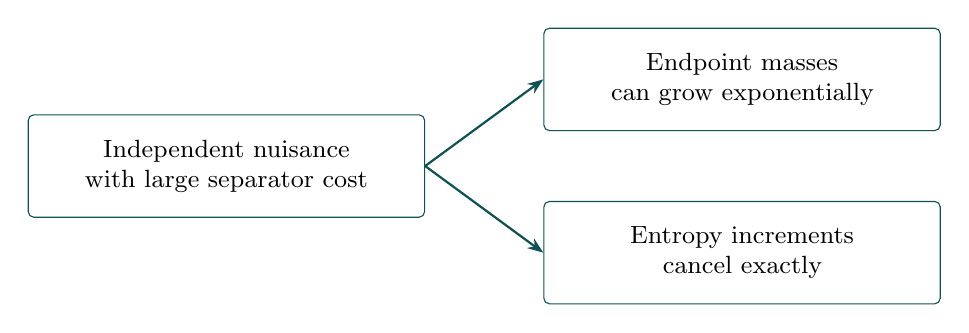
\begin{tikzpicture}[
 n/.style={draw=deepteal,rounded corners=2pt,align=center,
 text width=48mm,minimum height=13mm,font=\small},
 a/.style={-{Stealth[length=2mm]},deepteal,thick}]
 \node[n] (pad) {Independent nuisance\\with large separator cost};
 \node[n,right=15mm of pad,yshift=11mm] (mass) {Endpoint masses\\can grow exponentially};
 \node[n,right=15mm of pad,yshift=-11mm] (inc) {Entropy increments\\cancel exactly};
 \draw[a] (pad.east)--(mass.west);
 \draw[a] (pad.east)--(inc.west);
\end{tikzpicture}
\end{center}

The scope is exact independence. General strategies may correlate the added answers or workspace with the base questions. Then their entropy contribution can vary with the exposure, and \eqref{eq:cancellation} has not been proved. Identifying an appropriate invariant conditional term to subtract is a different and still open operation.

% End cancellation.tex


% Begin discussion.tex
\section{Scope and further questions}\label{sec:discussion}
The main probability theorem separates a conditional information budget from the method that produces it. Its sparse-test argument accumulates the individual squared benchmarks and permits a weighted amount of failure at every finite length. The small explicit constants record the proof accounting; no optimized numerical rate is claimed.

For commuting games, the precise unresolved input in the paper is \(\FR(K)\). Given that input, the passage to the scalar budget and the resulting product and threshold conclusions are fully proved. The density step uses only continuous finite-table inequalities after eliminating representation-dependent quantities. It does not identify commuting strategies with finite tensor strategies.

The positive-factor results locate a second boundary. Exact decompositions outside the disjoint-block class cannot guarantee subexponential one-sided masses uniformly over strategies, even when the tested success is one. Allowing small relative filter error does not fix that difficulty uniformly on all tested instances, as \cref{thm:filterNoGo} shows. These are representation obstructions, not lower bounds against general quadratic repetition. A semantic reduction can remove harmless answer padding: deterministic local maps preserve POVM completeness and between-player commutation, and maps in both winning directions preserve all product values.

The cancellation theorem offers a more direct constructive route. It shows that positive masses can be a poor proxy for the entropy differences actually used by a reconstruction argument. The excess separator information in an independent register can be present at every exposure stage and disappear from every increment. Extending that subtraction to question-correlated workspace would require a local conditional structure that the independent tensor example supplies for free.

Three questions remain particularly concrete. First, can an adaptive choice of tested coordinates, possibly after local semantic reduction, produce an answer-free information budget for general predicates? Second, can the conditional-relative-entropy and marginal-replacement approach of \cite{Jain} be implemented in standard form while preserving the local question references and the actual conditional law? That transfer alone retains the checked-answer charge and would not yet give a general quadratic theorem. Third, can one obtain a fully heterogeneous intrinsic rate proportional to
\[
 \sum_i\frac{\eps_i^3}{\eps_i+\kappa_i}
\]
without a uniform bound on \(\kappa_i/\eps_i\)? The present budget charges a tested coordinate to all remaining coordinates, so replacing the largest ratio by an average is not justified.

Finally, the fifth-power deviation in \cref{thm:main} is not shown optimal. Independent coordinate play already imposes the usual binary relative-entropy ceiling on homogeneous thresholds, and the line game prevents a universal improvement beyond the quadratic all-wins gap scale. Neither comparison determines the optimal heterogeneous threshold. No efficient finite-matrix compiler, physical advantage or new complexity classification follows from the probability theorem.

% End discussion.tex

\section*{Acknowledgements and AI use}
The mathematical ideas, constructions, proofs, and manuscript were developed by GPT-6 Astra, with additional AI assistance for review. Human input was minimal and consisted primarily of setting the research objectives and providing occasional feedback. GPT-6.1 Sol was used for independent constructions, mathematical review and literature checks.
\appendix

% Begin auxiliary.tex
\section{Finite information identities}\label{app:entropy}
This appendix supplies the elementary estimates used in the robust separator argument. All alphabets are finite.

\begin{lemma}[Conditional-entropy continuity]\label{lem:conditionalcontinuity}
If \(\TV(P_{CX},Q_{CX})\le\beta\le1/2\), then
\[
 |\Ent_P(X\mid C)-\Ent_Q(X\mid C)|
 \le\beta\log|\mathcal X|+h(\beta).
\]
The bound does not depend on \(|\mathcal C|\).
\end{lemma}
\begin{proof}
Take a maximal coupling of \((C,X)\) and \((C',X')\), with mismatch event \(B\) of probability \(\delta\le\beta\). Conditional on \(B=0\), the two pairs agree and have a common conditional law. Write its conditional entropy as \(H_0\). Since adding \(B\) to the conditioning can only decrease entropy,
\(\Ent_P(X\mid C)\ge(1-\delta)H_0\).
On the other side,
\[
 \Ent_Q(X'\mid C')
 \le\Ent(B)+(1-\delta)H_0+\delta\log|\mathcal X|.
\]
Subtract. Reversing the roles gives the absolute-value estimate with \(\delta\). Monotonicity of \(h\) on \([0,1/2]\) gives the displayed bound.
\end{proof}

\begin{lemma}[Binary discrimination entropy]\label{lem:binary}
Let \(L\) be a fair binary variable and, conditional on \(L\), let an observation have law \(p\) or \(q\) on \([m]\). If \(e=\frac12\sum_a\min(p_a,q_a)\), then
\[
 \tfrac12(\Ent(p)+\Ent(q))
 \le\log m-\log2+h(e).
\]
\end{lemma}
\begin{proof}
The maximum-likelihood estimate of \(L\) has error \(e\). Its error bit, together with the observation, determines \(L\), so
\(\Ent(L\mid X)\le h(e)\).
Now
\[
 \tfrac12(\Ent(p)+\Ent(q))
 =\Ent(X)-I(L;X)
 \le\log m-\log2+h(e).
\]
\end{proof}

\section{Checking the established unique-game comparison}\label{app:KRT}
We explain why \eqref{eq:KRT} follows from existing semidefinite machinery even for arbitrary commuting Hilbert-space strategies. The theorem numbers below refer to arXiv:0710.0655v3 \cite{KRT}.

For commuting projective measurements and a unit vector \(\psi\), put
\(u_a^x=P_a^x\psi\), \(v_b^y=Q_b^y\psi\), and realify their finite span. Within each question the vectors are orthogonal and their squared norms sum to one. Their cross inner products reproduce the game probabilities. Thus they are feasible for SDP~3, with the same objective. General finite POVMs can first be projectivized using separate finite ancillas with coefficients in the respective commuting algebras; this preserves cross commutation and all original correlations. Consequently
\[
 \omega_{\co}(G)\le s(G),
\]
where \(s(G)\) is the SDP~3 value.

Lemma~5.7 constructs a finite-dimensional tensor strategy from an SDP solution of value \(1-t\), with success at least \(1-2\sqrt{2t}-4t\). Set \(\eps=1-\omega_{\co}(G)\). Since such tensor strategies are commuting, \(t<\eps^2/16\) would imply
\[
 \eps\le2\sqrt{2t}+4t
 <(1/\sqrt2+1/4)\eps<\eps,
\]
using \(0<\eps\le1\). Hence \(s(G)\le1-\eps^2/16\).

Theorem~5.5 makes strictly feasible bipartite SDPs multiplicative. SDP~3 is strictly feasible by taking all of its vectors orthogonal with positive squared norms summing to one within each question. Section~5.3 and Remark~5.8 show that the bipartite product is a relaxation of the SDP of the product game, including products of different games. Iterating,
\[
 \omega_{\co}\left(\bigotimes_iG_i\right)
 \le\prod_i s(G_i)\le\prod_i(1-\eps_i^2/16).
\]
This proves the comparison. It does not assert equality of tensor and commuting values, and it applies to unique predicates rather than every projection predicate.

\Needspace{18\baselineskip}
\section{A guide to the hypotheses}\label{app:hypotheses}
For ease of reuse, the logical inputs are summarized here.
\begin{center}
\small
\begin{tabular}{p{39mm}p{99mm}}
\toprule
Result & Required input\\
\midrule
Weighted concentration &
The finite conditional budget \eqref{eq:budget} and
\(\kappa_i\le C_0\eps_i\); no game or independence assumption.\\[3pt]
Commuting consequence &
\(\FR(K)\), finite games with independent between-coordinate question laws, chosen exact rectangle partitions, and Lin's finite-table closure.\\[3pt]
Uniform mass obstruction &
Exact nonnegative bounded factorization on all mask entries; arbitrary global tensor factorizations allowed.\\[3pt]
Robust filter obstruction &
Classical conditional product prefilter law, bounded positive replacement filter, relative error at most \(\eps/8\), and the stated growing-alphabet family.\\[3pt]
Entropy cancellation &
Literal product state and coarse factors with a question-free independent nuisance register; base mass constant after flag averaging.\\
\bottomrule
\end{tabular}
\end{center}
\smallskip

The reconstruction hypothesis includes the operational local strategy, not merely a comparison between jointly indexed state descriptions. Its resource is fixed before the fresh inputs arrive and its POVMs are defined on every input pair. Approximation parameters may diverge in cost as the requested error decreases. No effective uniform bound follows from its quantifiers.

For the game consequence, the order of reasoning is important: first derive the scalar inequality for finite-tracial tables at fixed \(p_D>0\), then apply closure, and only then select or randomize the tested set. This prevents an unsupported convergence assertion for representation-dependent errors or unstable choices of tested coordinates.

% End auxiliary.tex


% Begin references.tex
\begin{thebibliography}{99}

\bibitem{Raz}
R. Raz.
A parallel repetition theorem.
\emph{SIAM Journal on Computing} \textbf{27}(3), 763--803, 1998.
\href{https://doi.org/10.1137/S0097539795280895}{doi:10.1137/S0097539795280895}.

\bibitem{Holenstein}
T. Holenstein.
Parallel repetition: Simplification and the no-signaling case.
\emph{Theory of Computing} \textbf{5}, Article 8, 141--172, 2009.
\href{https://doi.org/10.4086/toc.2009.v005a008}{doi:10.4086/toc.2009.v005a008}.

\bibitem{Rao}
A. Rao.
Parallel repetition in projection games and a concentration bound.
\emph{SIAM Journal on Computing} \textbf{40}(6), 1871--1891, 2011.
\href{https://doi.org/10.1137/080734042}{doi:10.1137/080734042}.

\bibitem{Unger}
F. Unger.
A probabilistic inequality with applications to threshold direct-product theorems.
\emph{Electronic Colloquium on Computational Complexity}, Report TR09-078, 2009.
\url{https://eccc.weizmann.ac.il/report/2009/078/}.

\bibitem{IK}
R. Impagliazzo and V. Kabanets.
Constructive proofs of concentration bounds.
\emph{Electronic Colloquium on Computational Complexity}, Report TR10-072, 2010.
\url{https://eccc.weizmann.ac.il/report/2010/072/}.

\bibitem{KRT}
J. Kempe, O. Regev, and B. Toner.
Unique games with entangled provers are easy.
\emph{SIAM Journal on Computing} \textbf{39}(7), 3207--3229, 2010.
\href{https://doi.org/10.1137/090772885}{doi:10.1137/090772885}.
Version used: \href{https://arxiv.org/abs/0710.0655v3}{arXiv:0710.0655v3}, 2009.

\bibitem{KR}
J. Kempe and O. Regev.
No strong parallel repetition with entangled and non-signaling provers.
\href{https://arxiv.org/abs/0911.0201v1}{arXiv:0911.0201v1}, 2009.

\bibitem{DS}
I. Dinur and D. Steurer.
Analytical approach to parallel repetition.
In \emph{Proceedings of the 46th Annual ACM Symposium on Theory of Computing},
624--633, 2014.
\href{https://doi.org/10.1145/2591796.2591884}{doi:10.1145/2591796.2591884}.
Version used: \href{https://arxiv.org/abs/1305.1979v3}{arXiv:1305.1979v3}, 2014.

\bibitem{DSV}
I. Dinur, D. Steurer, and T. Vidick.
A parallel repetition theorem for entangled projection games.
\emph{Computational Complexity} \textbf{24}, 201--254, 2015.
\href{https://doi.org/10.1007/s00037-015-0098-3}{doi:10.1007/s00037-015-0098-3}.
Version used: \href{https://arxiv.org/abs/1310.4113v2}{arXiv:1310.4113v2}, 2015.

\bibitem{LinTr}
J. Lin.
Tracially embeddable strategies: Lifting $\mathsf{MIP}^*$ tricks to
$\mathsf{MIP}^{\mathrm{co}}$.
\href{https://arxiv.org/abs/2304.01940v3}{arXiv:2304.01940v3}, 2025.

\bibitem{LinMIP}
J. Lin.
$\mathsf{MIP}^{\mathrm{co}}=\mathsf{coRE}$.
\href{https://arxiv.org/abs/2510.07162v1}{arXiv:2510.07162v1}, 2025.

\bibitem{Song}
Z. Song.
Parallel repetition for entangled games with gap exponent three.
\emph{Electronic Colloquium on Computational Complexity}, Report TR26-199, 2026.
\url{https://eccc.weizmann.ac.il/report/2026/199/}.

\bibitem{Jain}
R. Jain.
Parallel repetition for entangled games via conditional relative entropy.
\href{https://arxiv.org/abs/2610.21410v1}{arXiv:2610.21410v1}, 2026.

\bibitem{Wyner}
A. D. Wyner.
The common information of two dependent random variables.
\emph{IEEE Transactions on Information Theory} \textbf{21}(2), 163--179, 1975.
\href{https://doi.org/10.1109/TIT.1975.1055346}{doi:10.1109/TIT.1975.1055346}.

\bibitem{CPC}
P. W. Cuff, H. H. Permuter, and T. M. Cover.
Coordination capacity.
\emph{IEEE Transactions on Information Theory} \textbf{56}(9), 4181--4206, 2010.
\href{https://doi.org/10.1109/TIT.2010.2054651}{doi:10.1109/TIT.2010.2054651}.
Version used: \href{https://arxiv.org/abs/0909.2408v2}{arXiv:0909.2408v2}, 2010.

\bibitem{Cuff}
P. Cuff.
Distributed channel synthesis.
\emph{IEEE Transactions on Information Theory} \textbf{59}(11), 7071--7096, 2013.
\href{https://doi.org/10.1109/TIT.2013.2279330}{doi:10.1109/TIT.2013.2279330}.
Version used: \href{https://arxiv.org/abs/1208.4415v3}{arXiv:1208.4415v3}, 2013.

\bibitem{FP}
H. Fawzi and P. A. Parrilo.
Lower bounds on nonnegative rank via nonnegative nuclear norms.
\emph{Mathematical Programming} \textbf{153}(1), 41--66, 2015.
\href{https://doi.org/10.1007/s10107-014-0837-2}{doi:10.1007/s10107-014-0837-2}.
Version used: \href{https://arxiv.org/abs/1210.6970v2}{arXiv:1210.6970v2}, 2015.

\bibitem{Watts}
V. L. Watts.
Fractional biclique covers and partitions of graphs.
\emph{The Electronic Journal of Combinatorics} \textbf{13}(1), \#R74, 2006.
\href{https://doi.org/10.37236/1100}{doi:10.37236/1100}.

\bibitem{Pinto}
T. Pinto.
Biclique covers and partitions.
\emph{The Electronic Journal of Combinatorics} \textbf{21}(1), \#P1.19, 2014.
\href{https://doi.org/10.37236/3595}{doi:10.37236/3595}.
Version used: \href{https://arxiv.org/abs/1307.6363v2}{arXiv:1307.6363v2}, 2014.

\end{thebibliography}

% End references.tex

\end{document}
